\documentclass[12pt]{article}
\usepackage{graphicx}

\begin{document}
\begin{center}
\textbf\large{CHAPTER-7 \\ Straight Line and Pair of Straight Lines}

\end{center}

\section*{Section-A    [JEE Advanced/IIT-JEE]}
\section*{A    :  Fill in the Blanks}
\begin{enumerate}

\item  The area enclosed within the curves $|x|+|y|$ is.........\\
\item  $y=10^x$ is the reflection of $y=\log_10^x $ in the line whose equation is.........\\
\item The set of lines $ax+by+c=0$ where $3a+2b+4c=0$ is concurrent at the point..........\\
\item  Given the points A(0,4) and B(0,-4), the equation of the locus of the point P(x,y) such that$|AP-BP|=6$ is.............\\
\item  If $a,b and c$ are in A.P..then the straight line $ax+by+c=0$ will always pass through a fixed point whose coordinates are.........\\
\item  The orthocenter of the triangle formed by the lines $x+y=1, 2x+3y=6  and  4x-y+4=0$ lies in quadrant number............\\
\item Let the algebraic sum of the perpendicular distances from the points (2,0), (0,2) and (1,1)to a variable straight line be zero; then the line passes through a fixed point whose cordinates are.........\\
\item The vertices of a triangle are  A(-1,-7), B(5,1)and C(1,4). The equation of the bisector of the angle $\angle{ABC}$ is............\\

\end{enumerate}

\section*{B    :    True/False}
\begin{enumerate}

\item  The sraight line $5x+4y=0$ passes through the point of intersection of the straight lines $x+2y-10=0$ and $2x+5+6=0$.\\
\item The lines $2x+3y=19=0$ $9x+6y-17=0$ cut the coordinate axes in concyclic points.\\
\end{enumerate}

\section*{C  :   MCQ'S with One Correct Answer}
\begin{enumerate}

\item The points$(a,b),(0,0)(a,b)$ and $(a2.ab)$ are:
\begin{enumerate}
\item Collinear
\item Vertices of a parallelogram
\item Vertices of a rectangle
\item None of the above
\end{enumerate}
\item The point $(4,1)$ undergose the following three transformations successivvely.\\
i.Reflection about the line y=x\\
ii.Translation through a distance 2 unit along the positivedirection of x-axis.\\
iii. Rotation through an angle p/4 about the origin the counter clockwise direction.\\
then the final position of the point is given by the coordinates.
\begin{enumerate}
\item  $ [\frac{1}{\sqrt{2}},\frac{7}{\sqrt{2}}]$  
\item  $(-\sqrt{2}, \sqrt[7]{2})$  
\item  $[\frac{-1}{\sqrt{2}},\frac{7}{\sqrt{2}}]$
\item  $(\sqrt{2}, \sqrt[7]{2})$
\end{enumerate}
\item The straight lines $x+y=0, 3x+y-4=0,x+3y-4=0$ from a triangle which is 
\begin{enumerate}
\item isoscales 
\item equilateral
\item right angled  
\item  none of these 
\end{enumerate}
\item If $P=(1,0), Q=(-1,0) and R=(2,0)$ are three given
points, then  the locus  of the point S satisfying the relaion $SQ^2+SR^2=SP^2$, is
\begin{enumerate}
\item  a straight line parllel to x-axis  
\item  a circie passing hrough the origin 
\item  a circle with the center at the origin 
\item  a straight line parllel to y-axis
\end{enumerate}
\item Line L has intercepts a and b on the coordinate axes. Wen the axes are rotatwd through a given ange,keeingup the origin fixed,the same ine L has intercepts  pand q then
\begin{enumerate}
\item  $a^2=b^2=p^2=q^2$ 
\item $\frac{1}{a^2} +\frac{1}{b^2}= \frac{1}{p^2}=\frac{1}{q^2}$ 
\item  $a^2+p^2=b^2+q^2$ 
\item $\frac{1}{a^2}+\frac{1}{p^2}=\frac{1}{b^2}+\frac{1}{q^2}$
\end{enumerate}
\item If the sum of the distance of point from two perpendicular lines in a plane is 1,then its locu's is 
\begin{enumerate}
\item square 
\item  circle 
\item  straight line  
\item two intersecting lines
\end{enumerate}
\item The locus of the vaiable point whose distance from from $(-2,0)$ is 2/3 times it's distance from the line $x=\frac{-9}{2}$ is
\begin{enumerate}
\item elipse 
\item  parabola  
\item  hyperbola  
\item  none of the above
\end{enumerate}
\item The equation to a pair of  opposite sides of parallelogram are $x^2-5x+6=0$ and $y^2-6y+5=0$ the equations to it's diagonals are
\begin{enumerate}
\item $x+4y=13, y=4x-7$  
\item   $4x+y=13, 4y=x-7$ 
\item   $4x+y=13, y=4x-7$
\item $y-4x=13,y+4x=7$ 
\end{enumerate}
\item The orthocenter of the lines formed by $xy=0$ and $x+y=1$ is
\begin{enumerate}
\item  (1/2,1/2) 
\item   (1/3,1/3) 
\item    (0,0)
\item   (1/4,1/4)
\end{enumerate}
\item Let PQR be a rightangled isoscales triangle, right angled at $P(2,1)$ if the equation of the line QR is $2x+y=3$, then the equation representing the pair of line PQ and PR is
\begin{enumerate}
\item $3x^2-3y^2+8xy+20x+10y+25=0$
\item   $3x^2-3y^2+8xy-20x-10y+25=0$
\item   $3x^2-3y^2+8xy+10x+15y+20=0$
\item  $3x^2-3y^2-8xy-10x-15y-20=0$
\end{enumerate}
\item If $x_1,x_2,x_3$ as well as $y_1,y_2,y_3 $are in GP with the same common ratio, then the points $(x_1,y_1),(x_2,y_2)$ and $(x_3,y_3)$
\begin{enumerate}
\item lie on a straight line 
\item lie on a elipse 
\item lie on a circle  
\item  are vertices of trianngle 
\end{enumerate}
\item Let PS median of the tringle with vertices P(2,2), Q(6,1) and R(7,3). The equation of the line passing through (1,-1) and parllel to PS is.
\begin{enumerate}
\item $2x-9y-7=0$ 
\item   $2x-9y-11=0$ 
\item $2x+9y-11=0$
\item $2x+9y+7=0$
\end{enumerate}
\item  The incenter of the triangle with vertices $\frac{1}{\sqrt{3}}$,$(0,0)$ and $(2,0)$ is
\begin{enumerate}
\item $[1,\sqrt{3}/2]$ 
\item $\frac{2}{3}\,\frac{\sqrt{3}}{2}$ 
\item  $\frac{2}{3},\frac{\sqrt{3}}{2}$ 
\item  $[1,{1}{\sqrt{3}}]$
\end{enumerate}
\item The number of integer values of m, for which the x-coordinate of the of intersection of line $3x+4y=9$ and $y=mx+1$ is also an integer, is
\begin{enumerate}
\item  2 
 \item 0 
 \item  4   
 \item  1
 \end{enumerate}
\item  Area of parllelogram formed by the lines $y=mx$, $y=mx+1$,  $y=nx$ and  $y=nx+1$ equals
\begin{enumerate}
\item $\frac{\mid m+n\mid}{(m-n)^2}$
\item $\frac{2}{\mid m+n \mid}$
\item $\frac{1}{(\mid m+n \mid)}$
\item $\frac{1}{(\mid m-n\mid)}$
\end{enumerate}
 \item Let $0<a<\frac{\pi}{2}$ be fixed angle. If $P=(\cos\theta,\sin\theta)$, Q=$(\cos\alpha-\theta),(\sin\alpha-\theta)$, then Qis obtained from P by
 \begin{enumerate}
\item  clockwise wise rotation around origin through an angle $\alpha$
\item anticlockwise wise rotation around origin through an angle $\alpha$
\item reflection in the line through origin with slope $\tan\alpha$
\item reflection in the line through origin with slope $\tan\alpha/2$
\end{enumerate}
\item Let $P=(-1,0)$,$Q=(0,0)$ and $R=(3,\sqrt[3]{3})$ be three points.\\
Then the equation of the bisector of the angle PQR is
\begin{enumerate}
\item  $\frac{\sqrt{3}}{2x}+y=0$ 
\item  $(x+\sqrt{3}y=0)$
\item  $\sqrt{3}x+y=0$ 
\item $x+\frac{\sqrt{3}}{2y}=0$
\end{enumerate}
\item A straight line through the origin O meets the parallel lines $4x+2y=9$ and $2x+y+6=0$ at points P and Q respectively. Then the point O divides the segment PQ in the ratio
\begin{enumerate}
\item $1:2$   
\item$3:4$
\item  $2:1$ 
\item$4:3$ 
\end{enumerate}
\item The number of integral points(integral points means both the coordinates should be integer) exactly in the interior of the triangle with vertices is $(0,0)(0,21)$ and $(21,0)$ is
\begin{enumerate}
\item 133  
\item 190  
\item 233 
\item 105
\end{enumerate}
\item Orthocenter of triangle with vertices $(0,0)(3,4)$ and $(4,0)$ is 
\begin{enumerate}
\item $[3,\frac{5}{4}]$ 
\item$[3,12]$   
\item $[3,\frac{3}{4}]$ 
\item$[3,9]$
\end{enumerate}
\item Aear of the triangle formed by the line $x+y=3$ and angle bisectors of the pair of straight lines $x^2-y^2+2y=1$
\begin{enumerate}
\item  2 sq. units  
\item  4 sq. units 
\item  6 sq. units    
\item 8 sq. units
\end{enumerate}
\item Let $O(0,0),P(3,4),Q(6,0)$ be the vertices of the tiangles OPQ. The point R inside the triangle OPQ is such that the triangles OPR,PQR,,OQR are of equal area. The coordinates of R are 
\begin{enumerate}
\item $[\frac{4}{3}, 3]$   
\item $[3, \frac{2}{3}]$  
\item   $[3, \frac{4}{3}]$  
\item $[\frac{4}{3}, \frac{2}{3}]$
\end{enumerate}
\item A straight line through the point $(3,2)$ inclined at an angle $ 60^\circ $  to the line $\sqrt{3}x+y=1$. If L also intersects the x axis, then the equation of L is 
\begin{enumerate}
\item  $y+\sqrt{3}+2+\sqrt[3]{3}=0$
 \item  $y-\sqrt{3}+2+\sqrt[3]{3}=0$ 
 \item  $\sqrt{3}y-x+3+\sqrt[2]{3}=0$  
 \item  $\sqrt{3}y+x-3+\sqrt[2]{3}=0$
\end{enumerate}

\end{enumerate}

\section*{D   :  MCQ'S with One or More Than One Correct Answer}
\begin{enumerate}

\item Three lines $px+qy+r=0$, $qx+ry+p=0$ and $rx+py+q=0$ are concurrent if 
\begin{enumerate}
\item $p+q+r=0$
\item $p^2+q^2+r^2=qr+rp+pq$
\item $p^3+q^3+r^3=3pqr$
\item none of these
\end{enumerate}
\item The points $[0,\frac{8}{3}]$,$[1,3]$ and $[82,30]$ are vertices of
\begin{enumerate}
\item an obtuse angle triangle
\item an acute angle triangle 
\item  a right angled triangle
\item  an isoscales triangle
\item none of these
\end{enumerate}
\item All points lying inside the triangle are formed by the points$(1,3)$,$(5,0)$ and $(-1,2)$ satisfy
\begin{enumerate}
\item  $3x+2y\ge=0$
\item $2x+3y-13\ge=0$
\item  $2x-3y-12\le=0$
\item $-2x+y\ge=0$
\item none of these
\end{enumerate}
\item A vector $\bar{a}$ has components of 2p and 1 with respect to a rectangular cartesian system. This system is rotted through a certain angle about origin in the counter clockwise sense. If,with respect the new system,$\bar{a}$ has components $p+1$ and 1, then
\begin{enumerate}
\item $p=0$  
\item  $p=1$ or $p=-1/3$  
\item $p=-1$ or $p=1/3$ 
\item  $p=1$ or $p=-1$
\item none of these.
\end{enumerate}
\item  If $P(1,2),Q(4,6),R(5,7)$ and $S(a,b)$ are the vertices of a parallelogram PQRS, then
\begin{enumerate}
\item $a=2,b=4$
\item $a=3,b=4$ 
\item $a=2,b=3$
\item $a=3,b=5$
\item none of these
\end{enumerate}
\item The diagonals of a parallelogram PQRS are along the lines $x+3y=4$ and $6x-2y=7$ then PQRS must be a.
\begin{enumerate}
\item rectangle
\item square
\item cyclic quadrilateral
\item rhombus
\end{enumerate}
\item If the vertices P,Q,R of a triangle PQR are rational points, which of the following points of the triangle PQR is (are) always rational point(s)?
\begin{enumerate}
\item centroid 
\item  incenter
\item circumcenter 
\item orthocenter
(A rational point is a point both of whose coordinates are rational numbers.)
\end{enumerate}
\item  Let $L_1$ be a straight line passing through the origin and $L_2$ be the straight line $x+y=1$. If the intercepts made by the circle $x^2+y^2-x+3y=0$ on $L_1$ and $L_2$ are equal, then which of the equation can represents $L_1$?
\begin{enumerate}
\item $x+y=0$   
\item $x-y=0$ 
\item $x+7y=0$  
\item $x-7y=0$
\end{enumerate}
\item  For $a>b>c>0$,the distance between (1,1)and the point of intersection of the lines $ax+by+c=0$ and $ay+c=0$ is less than $\sqrt[2]{2}$. Then
\begin{enumerate}
\item $a+b-c>0$ 
\item $a-b+c<0$
\item $a+b-c>0$
\item $a+b-c<0$
\end{enumerate}

\end{enumerate}
\section*{E  :  Subjective Problems}
\begin{enumerate}


\item  A straight line segment of length l moves with it's ends on two mutually perpendicular lines. Find the locus of the point which divides the line segment in the ratio $1:2$.
\item The area of triangle is 5. Two of it's vertices are A(2,1) and B(3-2). The third vertex C lies on $y=x+3$. Finf C.
\item One side of the rectangle lies along the line $4x+7y+5=0$. Two of it's vertices are (-3,1) and (1,1). Find the equation of the other two sides.
\item(a) Two vertices of a triangle are (5,-1) and (-2,3) If the orthocenter of the triangle is the origin,find the coordinates of the third point.
(b) Find the equation of the line which bisects the obtuse angle between the lines $x-2y+4=0$ and $4x-3y+2=0$\\
\item  A straight line L is perpendicular to the line $5x-y=1$. The area of the triangle formed by the line L and the coordinate axes is 5. Find the equation of the line.\\
\item The end A,B of a straight line segment of constant length c slide upon he fixed rectangular axes $(X,Y)$ respectively. If a rectanle OAPB are completed, then show that the locus of the foot of the perpendicular drawn from P to AB is $x^(\frac{2}{3})+y^(\frac{2}{3})=c^(\frac{2}{3})$.\\
\item The vertices of the triangle are $[at_1t_2,a(t_1+t_2)]$,$[at_1t_3,a(t_1+t_3)]$ and $[at_3t_4,a(t_3+t_4)]$. Find the orthocenter of the triangle.\\
\item The coordinates of A,B,C are  (6,3),(3,5),(4,2) respectively, and P is any point (x,y). Show that the ratio of the area of the triangle $\triangle PBC$ and $\triangle ABC $ is $\mid\frac{(x+y-2)}{7}\mid$\\
\item Two equal sides of a isoscales triangle are given by the equations $7x-y+3=0$ and $x+y-3=0$ and it's third side passes through the point $(1,10)$. Determaine the equation of the third side.\\
\item One of the diametes of the circle circumscribing the rectangle ABCD is $4y=x+7$. If A and B are the ponts $(-3,4) and (5,4)$ respetively then find the area of the rectangle.\\
\item Two sides of a rhombus ABCD are parallel to the lines $y=x+2 and y=7x+3$. If the diagonals of the rhombus intersects at the point $(1,2)$ and the vertex A on the y axis, find the possible coordinates of A.\\
\item Lines $L_1=ax+by+c=0$ and $L_2=lx+my+n=0$ intersects at the point P and make an angle $\theta$ with each other. Find the equation of a line L different from $L_2$ which passes through P and makes the same angle $\theta$ with $L_1$.\\
\item Let ABC be a triangle with $AB-AC$.r If D is the pont of BC, E is the foot of the perpendicular drawn from D to AC and F the mid point of DE, prove that AF is perpendicular to BE.\\
\item Sraight lines $3x+4y-5$ and $4x+3y-5$ intersects at the point A. Points B and C 
are choosen on these two lines such that $AB=AC$. Determine the possible equaton of the line BC passing through the point (1,2).\\
\item A line cuts the x-axis at A(7,0) and the y-axis at B(0,5). A variable line PQ drawn perpendicular to AB cutting the x-axis  in P and y-axis in Q. If AQ and BP intersets at R, find the locus of R.\\
\item Find the equation of the line passing through the point (2,3)and intersects of length 2 units between the lines $y+2x=3$ and $y+2x=5$.\\
 
 \begin{figure}[h]
\centering
    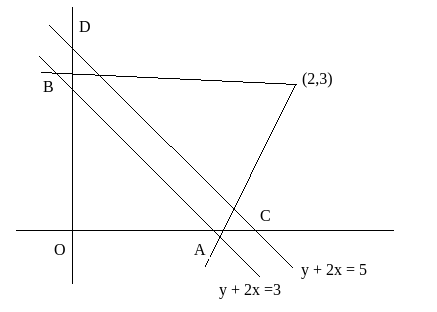
\includegraphics[width=4cm, height=2cm]{fig.png}
     \end{figure}
     
\newpage
\item Show that all chords of the curve  $2x^2-y^2-2x+4y=0$. Which subtend a right angle at the origin. Passes through a fixed point. Find the coordinates of the point.\\
\item Determine all values of a for which the point $(a, a^2)$ lies inside the triangle formed by the lines\\
$2x+3y-1=0$\\
$x+2y-1=0$\\
$5x-6y-1=0$\\
\item Tangent at a point $P_1$ [other than (0,0)] on the curve $y-x^3$ meets the curve again at $P_2$. The tangent at $P_1$ meets the curve at $P_2$ and so on. Show that the abscissae of $p_1+p_2+p_3+.....+p_n$ form a G.P. Also find the ratio.\\
\item A line through $A(5,4)$ meets the line $x+3y+2=0$ $2x+y+4=0$ and $x-y-5=0$ at points B,C and D respectively. If    $\frac{15}{AB}^2+\frac{10}{AC}^2-\frac{6}{AD}^2$, find the equation of the line.\\
\item A triangle PQRS has it's side PQ parallel to the line $y-mx$ and vertices P,Q and S on the lines $y-a$,$ x-b$ and $x--b$, respectively find the locus of the vertex R.\\
\item Using co-ordinate geometry prove that the three altitudes of any triangle are concurrent\\
\item For points $P=(x_1,Y_1)$ and $Q=(x_2,y_2)$ of the coordinate palne, a new distance $d(P,Q)$ is defined by $d(P,Q)=\mid x_1-x_2\mid + \mid y_1-y_2\mid$. Let $O=(0,0)$  and $A=(3,2)$. Prove that the set of points in the first quadrant which are equidistance (with to line new distance) from O and A consists of the union of line segment of finite length and an infinite ray. Sketch this set in a labelled diagram.\\
\item Let ABC and PQR be any two triangles in the same plane. Assume that the perpendicular from the points A,B,C to the sides QR, RP, PQ respectively are concurrent. Using vector methods or otherwise, prove that the perpendiculars from P,Q,R to BC, CA, AB  respectively are also concurrent.\\
\item Let a,b,c are real numbers with $a^2+b^2+c^2=1$. Show that the equation\\
$\Bigg |ax-by-c\hspace{1cm}bx+ay\hspace{1cm} cx+a\\
bx+ay  \hspace{1cm}ax+by-c  \hspace{1cm}cy+b\\
cx+a   \hspace{1cm} cy+b  \hspace{1cm}  ax-by+c\Bigg |$ =0\\
represents a straight line.\\
\item A straight line L through the origin meets the lines $x+y+1$ and $x+y=3$ at P and Q respectively. Through  P and Q two straight lines $L_1 and L_2$ intersects at R . Show that the locus of R, as L varies, is a staight line.\\
\item A straight line negative slope passes through the points $(8,2)$ cuts the positive coordnate axes at points P and Q. Find the absolute minimum value of OP+OQ, as L varies . Where O is the origin.\\
\item The area of the triangle formed by the intersection of a line parallel to x-axis and passing through $p(h,k)$ with the lines $y-x$ and $x+y-2$ is $4h^2$. Find the locus of the point .\\
\end{enumerate}

\section*{H   : Assertion and Reason Type Questions}

\begin{enumerate}

\item Lines $L_1: Y-X=0$ and $L_2 :2x+y=0$ intersects the line $l_3:y+2=0$ at P and Q, respectively. The bisector of the acute angle between $L_1 and L_2$ intersects $L_3$ at R.\\
STATEMENT-1 : The ratio $PR:RQ$equals $\sqrt[2]{2}:\sqrt{5}$. because \\
STATEMENT-2 :In any triangle, bisector of an angle divides the triangle into two triangles.
\begin{enumerate}
\item Statement-1 is True, Statement-2 is True;Satement-2 is not a correct explaination for Statement-1
\item Statement-1 is True, Statement-2 is True;Satement-2 is NOT a correct explaination for Statement-1
\item Statement-1 is True, Statement-2 is False
\item Statement-1 is False, Statement-2 is True
\end{enumerate}
\end{enumerate}

\section*{I    :     Integer Value Correct Type }
\begin{enumerate}

\item For a point P in the plane, let $d_1(p)$ and $d_2(p)$ be the distance of a point P
from the lines $x-y=0$ and $x=y=0$ respectively. The area of the region R consistes of all points P lying in the first quadrant of the plane and satisfying $2\leq d_1(p)+d_2(p)\leq$, is
\end{enumerate}

\section*{Section-B   [JEE Main/AIEE]}
\begin{enumerate}
\item A triangle with vertices$(4,0),(-1,-1 ),(3,5)$ is
\begin{enumerate}
\item isoscales and right angled
\item isoscales  but not right angled
\item right angled but not isoscales 
\item neither right angled nor isoscales 
\end{enumerate}
\item Locus of mid point of the portion between the axes of $x\cos\alpha+y\sin\alpha=p$. Where p is constant is.
\begin{enumerate}
\item $x^2+y^2=\frac{4}{p^2}$ 
\item $x^2+y^2=4p^2$
\item$\frac{1}{x^2}+\frac{1}{y^2}=\frac{2}{p^2}$ 
\item $\frac{1}{x^2}+\frac{1}{y^2}=\frac{4}{p^2}$ 
\end{enumerate}
\item If the pair of lines $ax^2+2hxy+by^2+2gx+2fy+c=0$ intersects on the y-axis then
\begin{enumerate}
\item $2fgh=bg^2+ch^2$ 
\item $bg^2\neq ch^2$
\item $abc=2fgh$
\item none of these
\end{enumerate}
\item The pair of lines represented by $3ax^2+5xy+(a^2-2)y^2=0$ are perpendicular to each other for 
\begin{enumerate}
\item two values of a
\item $\forall a$
\item for one value of a 
\item for no values of a
\end{enumerate}
\item A square of side a lies above the x-axis and has one vertex at the origin. The side passing through the origin makes an angle $\alpha \left[ 0<a<\frac{\Pi}{4}]\right]$ with the positive direction of x-axis. The equation of it's diagonal passing through the origin is 
\begin{enumerate}
\item $y(\cos\alpha+\sin\alpha)+x(\cos\alpha-\sin\alpha)$=a
\item $y(\cos\alpha-\sin\alpha)-x(\sin\alpha-\cos\alpha)$=a
\item $y(\cos\alpha+\sin\alpha)+x(\sin\alpha-\cos\alpha)$=a
\item $y(\cos\alpha+\sin\alpha)+x(\sin\alpha+\cos\alpha)$=a
\end{enumerate}
\item If the pair of straight lines $x^2-2pxy-y^2=0$ and $x^2-2qxy-y^2=0$ be such that each pair bisects the angle between the other pair, then 
\begin{enumerate}
\item $pq=-1$  
\item $p=q$ 
\item $p=-q$  
\item $pq=1$
\end{enumerate}
\item Locus of centroid of the triangle whose vertices are $(a\cos t, a\sin t)$, $(a\sin t,-b\cos t)$ and (1,0) where t is a parameter, is 
\begin{enumerate}
\item$(3x+1)^2+(3y)^2=a^2-b^2$
\item $(3x-1)^2+(3y)^2=a^2-b^2$
\item $(3x-1)^2+(3y)^2=a^2+b^2$
\item $(3x+1)^2+(3y)^2=a^2+b^2$
\end{enumerate}
\item If $x_1,x_2,x_3$ and $y_1,y_2,y_3$ are both in G.P with the same common ratio then the points $(x_1,y_1),(x_2,y_2)$ and $(x_3,y_3)$
\begin{enumerate}
\item are vertices of a triangle
\item lies on a straight line
\item lies on elipse
\item lies on circle
\end{enumerate}
\item If the equation of the locus of a equidistance from the point $(a_1,b_1)$ and $(a_2,b_2)$ is $(a_1-b_2)x+(a_1-b_2)y+c=0$, then the value of 'c' is
\begin{enumerate}
\item $\sqrt{a_1^2+b_1^2-a_2^2-b_2^2}$
\item $\frac{1}{2}(a_2^2+b_2^2-a_1^2-b_1^2)$
\item $a+1^2-a_2^2+b_1^2-b_2^2$
\item $\frac{1}{2}(a_1^2+a_2^2+b_1^2+b_2^2)$
\end{enumerate}
\item Let $A(2,-3)$ and $B(-2,3)$ be vertices of a triangle ABC. If the centroid of this triangle moves on the line $2x+3y=1$, then the locus of the vertex C is in the line 
\begin{enumerate}
\item $3x-2y=0$
\item $2x-3y=7$ 
\item $3x+2y=5$ 
\item $2x+=3y=9$
\end{enumerate}
\item The equation of the straight line passing through the point (4,3) and making intercepts on the coordinate axes whose sum is -1 is 
\begin{enumerate}
\item $\frac{x}{2}-\frac{y}{3}=1$ and $\frac{x}{-2}+\frac{y}{1}=1$
\item $\frac{x}{2}-\frac{y}{3}=-1$ and $\frac{x}{-2}+\frac{y}{1}=-1$
\item $\frac{x}{2}+frac{y}{3}=1$ and $\frac{x}{2}+\frac{y}{1}=1$
\item $\frac{x}{2}+\frac{y}{3}=1$ and $\frac{x}{-2}+\frac{y}{1}=-1$
\end{enumerate}
\item If the sum of the slopes of the lines given by $x^2-2cxy-7y^2=0$ is four times the product c has the value
\begin{enumerate}
\item -2 
\item -1 
\item  2 
\item  1
\end{enumerate}
\item If one of the lines given by $6x^2-xy+4cy^2=0$ is $3x+4y=0$, then c equals 
\begin{enumerate}
\item -3 
\item -1 
\item  3 
\item  1
\end{enumerate}
\item The line parallel to the x-axis and passing through the intersection of the lines $ax+2by+3b=0$ and $bx-2ay-3a=0$, where $(a,b) \neq (0,0)$
\begin{enumerate}
\item below the x-axis at a distance of $\frac{3}{2}$ from it
\item below the x-axis at a distance of $\frac{2}{3}$ from it
\item above the x-axis at a distance of $\frac{3}{2}$ from it
\item above the x-axis at a distance of $\frac{2}{3}$ from it
\end{enumerate}
\item If a vertex of a triangle is (1,1) and the mid point of two sides of this vertex are (-1,2) and (3,2) then the centroid of the triangle is 
\begin{enumerate}
\item $\left[-1,\frac{7}{3}\right]$ 
\item $\left[ \frac{-1}{3},\frac{7}{3}\right]$ 
\item $\left[1,\frac{7}{3}\right]$  
 \item $\left[ \frac{1}{3},\frac{7}{3}\right]$ 
\end{enumerate}
\item A straigjt line through point $A(3,4)$ is such that it's intercept between the axes is bisected at A. It's equation is
\begin{enumerate}
\item  $x+y=7$ 
\item $3x-4y+7=0$  
\item $4x+3y=24$ 
\item $3x+4y=25$
\end{enumerate}
\item If $(a,a^2)$ falls inside the angle made by the lines $y= \frac{x}{2}, x>0$ and $y=3x, x>0$, then a belong to 
\begin{enumerate}
\item $\left[ 0,\frac{1}{2}\right] $ 
\item $(3,\infty)$ 
\item $\left[\frac{1}{2},3\right]$ 
\item $\left[-3,\frac{1}{2}\right]$
\end{enumerate}
\item Let $A(h,k)$ and $B(1,1)$ and $C(2,1)$ be the vertices of a right angle triangle with AC as it's hypotenuse. If the area of the triangle is 1 square unit, then the set of values which 'k' can taken is given by
\begin{enumerate}
\item $(-1,3)$ 
\item $(-3,-2)$
\item$(1,3)$ 
\item $(0,2)$
\end{enumerate}
\item Let $P=(-1,0),Q=(0,0) and R=(3,\sqrt[3]{3})$ be three points. The equation of the bisector of the angle PQR is 
\begin{enumerate}
\item $\frac{\sqrt{3}}{2}x+y=0$ 
\item $x+\sqrt{3}y=0$ 
\item $\sqrt{3}x+y=0$ 
\item $x+\frac{\sqrt{3}}{2}y=0$.
\end{enumerate}
\item If one of the lines of $my^2+(1-m^2)xy-mx^2=0$ is a bisector of the angle between the lines $xy=0$, then m is
\begin{enumerate}
\item 1  
\item 2 
\item $\frac{-1}{2}$ 
\item -2
\end{enumerate}
\item The perpendicular bisector of the line segment joning $P(1,4)$ and $Q(k,3)$ has y-intercept -4. Then a possible value of k is
\begin{enumerate}
\item  1 
\item  2 
\item -2 
\item -4
\end{enumerate}
\item The shortest distance between the line $y-x=1$ and the curve $x=y^2$ is 
\begin{enumerate}
\item $\frac{\sqrt{2}{3}}{8}$ 
\item $\frac{\sqrt{3}{2}}{5}$ 
\item $\frac{\sqrt{3}}{4}$ 
\item $\frac{\sqrt{3}{2}}{8}$.
\end{enumerate}
\item The lines $p(p^2+1)x-y+q=0$ and $(p^2+1)^2x+(p^2+1)y+2q=0$ are perpendicular to a common line for 
\begin{enumerate}
\item exactly one value of p
\item exactly two values of p
\item more than two values of p
\item no value of p
\end{enumerate}
\item Three distinct points A,B and C are given i the 2-dimentional coordinates plane such that the ratio of the  distance of any one of them from the point (1,0) to the distance from the point (-1,0) is equal to $\frac{1}{3}$. Then the circumcenter of the triangle ABC is at the point;
\begin{enumerate}
\item $[\frac{5}{4} ,0]$ 
\item $[\frac{5}{2} ,0]$ 
\item$[\frac{5}{3} ,0] $
\item (0,0)
\end{enumerate}
\item The line L given by $\frac{x}{5}+\frac{y}{b}=1$ passes through the point (13,32). The line K is parallel L and has the equation $\frac{x}{c}+\frac{y}{3}=1$. Then the distance between L and K is 
\begin{enumerate}
\item $\sqrt{17}$  
\item$\frac{17}{\sqrt{15}}$ 
\item$\frac{23}{\sqrt{17}}$ 
\item $\frac{23}{\sqrt{15}}$
\end{enumerate}
\item The line $L_1:y-x=0$ and $L_2: 2x+=y=0$ intersects the line $L_3: y+2=0$ at P and Q respectively. The bisector of the acute angle between $L_1 and L_2$ intersects $L_3$ at R
STATEMENT-1: The ratio PR;RQ equals $\sqrt[2]{2}:\sqrt{5}$\\
 STATEMENT-2: In any triangle,bisector of an angle divides the triangle into two similar triangles.
 \begin{enumerate}
\item Statement-1 is True, Statement-2 is True,Statement-2 is not a correct explaination for the Statement-1.
\item Statement-1 is True, Statement-2 is False
\item Statement-1 is False, Statement-2 is True
\item Statement-1 is True, Statement-2 is True,tatement-2 is correct explaination for the Statement-1.
\end{enumerate}
\item  If the line $2x +y=k$ passes through the point which divides the line segment joining the points $(1,1)$ and (2,4) in the ratio $3:2$,then k equals:

\begin{enumerate}
\item $\frac{29}{5}$ 
\item 5 
\item 6 
\item $\frac{11}{5}$
\end{enumerate}
\item  A ray of light along $x+\sqrt{3}y=\sqrt{3}$ get reflected upon reaching x-axis, the equation of the reflected ray is
\begin{enumerate}
\item $y=x+\sqrt{3}$ 
\item $\sqrt{3}y=x-\sqrt{3}$ 
\item $y=\sqrt{3}x-\sqrt{3}$ 
\item $\sqrt{3}y=x-1$ 
\end{enumerate}
\item  The coordinate of the incenter of the triangle that has the coordinates of mid points of it's sides as (0,1) (1,1) and (1,0) is;
\begin{enumerate}
\item $2+\sqrt{2}$
\item $2-\sqrt{2}$ 
\item $1+\sqrt{2}$ 
\item $1-\sqrt{2}$
\end{enumerate}
\item  Let PS e the median of the triangle with vertices $P(2,2)$,$Q(6,-1)$ and $R(7,3)$. The equation of the line passing through (1,-1)and parallel to PS is:
\begin{enumerate}
\item $4x+7y+3=0$ 
\item $2x-9y+11=0$ 
\item $4x-7y+11=0$ 
\item $2x+7y+9=0$ 
\end{enumerate}
\item  Let a,b,c and d be non-zero numbers. If the point of intersection of the lines $4ax+2ay+c=0$ and $5bx+2by+d=0$ lies in the fourth quadrant and eqidistance from the two axes then 
\begin{enumerate}
\item $3bc_2ad=0$  
\item $3bc+2ad=0$
\item $2b-3ad=0$ 
\item $2bc+3ad=0$
\end{enumerate}
\item  The number of points, having both co-ordinates as integers, that lie in the interior of the triangle ith vertices (0,0)(0,41) and(41,0)is.
\begin{enumerate}
\item 820 
\item 780 
\item 901 
\item 861\\
\end{enumerate}
\item  Two sides  of a rhombus are alon the lines, $x-y+1=0$ and $7x+y-5=0$. If it's diagoals intersect at(-1,-2), then which one of the following is a vertex of this rhombus?
\begin{enumerate}
\item $\left[ \frac{1}{3},\frac{8}{3}\right]$ 
\item $\left[ \frac{10}{3},\frac{7}{3}\right]$ 
\item $(-3,-9)$ 
\item $(-3,-8)$
\end{enumerate}
\item   A straight the thrugh a fixed point (2,3)intersects the coordinate axes at distinct point P  and Q. If O is the origin and the rectangle OQPR is completed, then the locus of R is:
\begin{enumerate}
\item $2x+3y=xy$ 
\item $3x+2y=xy$ 
\item $3x+2y=6xy$ 
\item $3x+2y=6$
\end{enumerate}
\item  consider the set of all lines $px+qy+r=0$ such that $3p+2q+4r=0$. Which one of the following statements is true?
\begin{enumerate}
\item The lines are concurent at the point $\left[ \frac{3}{4}\frac{1}{2}\right] $.\\
\item Each the line passes through the origin.\\
\item The lines are parallel.\\
\item The lines are not concurrent.\\
\end{enumerate}
\item  Slope of line passing through $P(2,3)$ and intersecting the line $x+y=7$ at a distance of 4units from  P,  is :
\begin{enumerate}
\item $\frac{1-\sqrt{5}}{1+\sqrt{5}}$
\item $\frac{1-\sqrt{7}}{1+\sqrt{7}}$
\item $\frac{\sqrt{7}-1}{\sqrt{7}+1}$
\item$\frac{\sqrt{5}-1}{\sqrt{5}+1}$
\end{enumerate}
\end{enumerate}

\end{document}